% Figure 6: editable LaTeX layout.
% Change \figuresixpanelwidth or the tabular spacing below to adjust the layout.
\begin{figure}[!ht]
    \centering
    \begingroup
    \newlength{\figuresixpanelwidth}
    \setlength{\figuresixpanelwidth}{0.31\textwidth}

    \tikzset{
        figuresixcallout/.style={
            fill=white,
            fill opacity=0.86,
            text opacity=1,
            rounded corners=0.8pt,
            inner sep=1.2pt,
            align=center,
            font=\sffamily\bfseries\fontsize{5.8}{6.3}\selectfont
        },
        figuresixarrow/.style={
            ->,
            >=stealth,
            draw=black!70,
            line width=0.45pt
        }
    }

    \newcommand{\figuresixlabel}[2]{%
        {\sffamily\bfseries\fontsize{8.5}{9.5}\selectfont
         (#1) $\theta_c=#2^{\circ}$}%
    }

    \newcommand{\figuresixpanel}[3]{%
        \begin{tabular}[t]{@{}c@{}}
            \includegraphics[width=\figuresixpanelwidth]{#1}\\[-1pt]
            \figuresixlabel{#2}{#3}
        \end{tabular}%
    }

    \newcommand{\figuresixpanela}{%
        \begin{tabular}[t]{@{}c@{}}
            \begin{tikzpicture}
                \node[anchor=south west,inner sep=0] (figuresixaimage) at (0,0)
                    {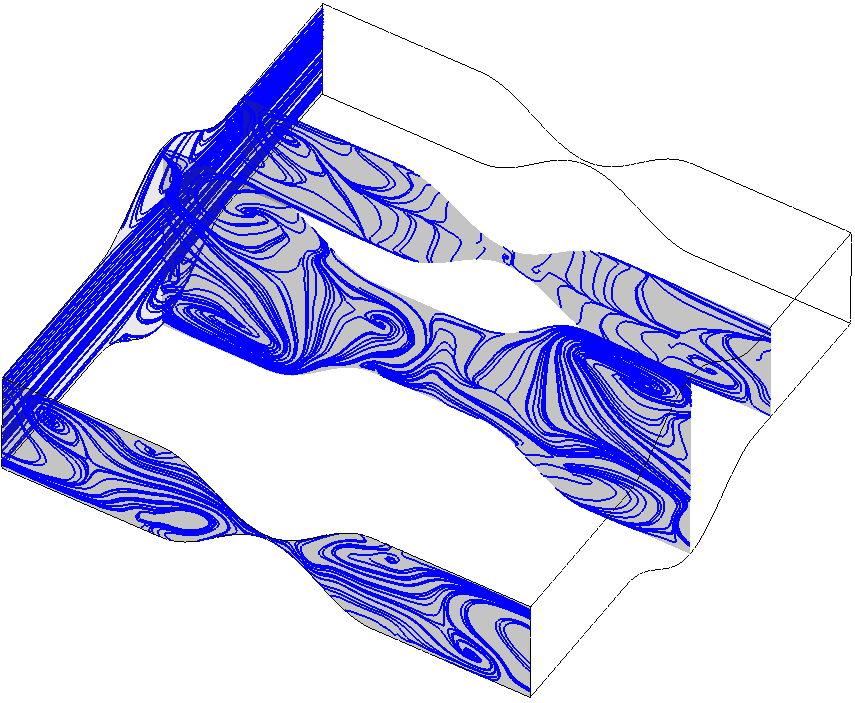
\includegraphics[width=\figuresixpanelwidth]{image_2/Figure7/CA_0deg_2D_stream.png}};
                \begin{scope}[x={(figuresixaimage.south east)},y={(figuresixaimage.north west)}]
                    \node[figuresixcallout] (figuresixwake) at (0.48,0.78)
                        {Wake\\recirculation};
                    \draw[figuresixarrow] (figuresixwake.south west) -- (0.31,0.47);
                \end{scope}
            \end{tikzpicture}\\[-1pt]
            \figuresixlabel{a}{0}
        \end{tabular}%
    }

    \newcommand{\figuresixpanelc}{%
        \begin{tabular}[t]{@{}c@{}}
            \begin{tikzpicture}
                \node[anchor=south west,inner sep=0] (figuresixcimage) at (0,0)
                    {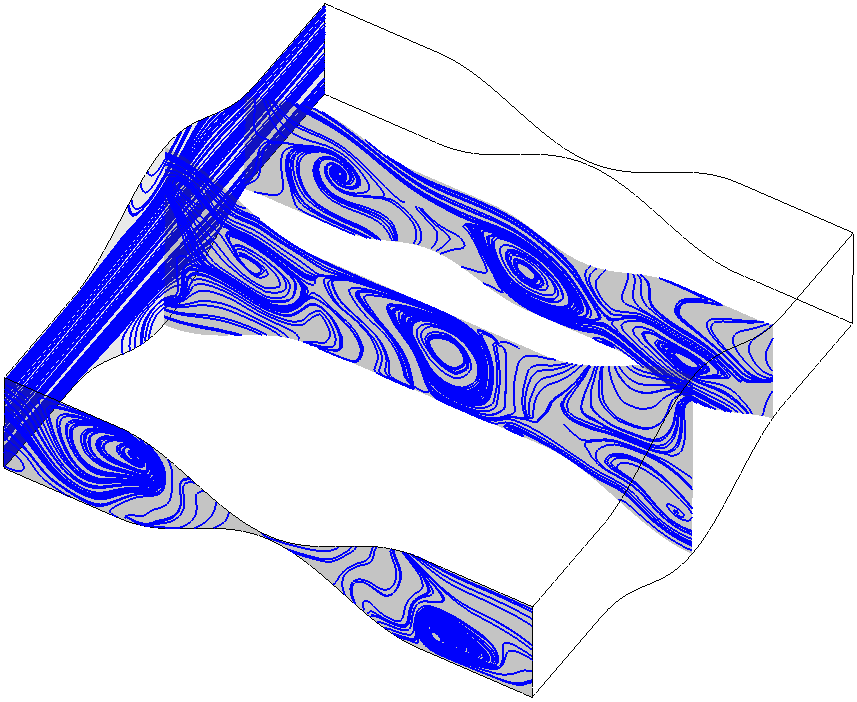
\includegraphics[width=\figuresixpanelwidth]{image_2/Figure7/CA_45deg_2D_stream.png}};
                \begin{scope}[x={(figuresixcimage.south east)},y={(figuresixcimage.north west)}]
                    \node[figuresixcallout] (figuresixreattach) at (0.58,0.79)
                        {Disturbed /\\reattaching flow};
                    \draw[figuresixarrow] (figuresixreattach.south) -- (0.55,0.49);
                \end{scope}
            \end{tikzpicture}\\[-1pt]
            \figuresixlabel{c}{45}
        \end{tabular}%
    }

    \begin{tabular}[c]{@{}c@{\hspace{0.06in}}c@{\hspace{0.06in}}c@{}}
        \figuresixpanela &
        \figuresixpanel{image_2/Figure7/CA_22.5deg_2D_stream.png}{b}{22.5} &
        \figuresixpanelc
    \end{tabular}
    \endgroup
    \caption{2D streamlines of CPHE at representative capsule angles ($\theta_c=0\degree$, $22.5\degree$, and $45\degree$).}
    \label{figure6}
\end{figure}
